\documentclass[10pt,a4paper]{article}
 
\usepackage[utf8x]{inputenc}
\usepackage[norsk]{babel}
\usepackage[T1]{fontenc,url}
\usepackage[hang,small,bf]{caption}
\usepackage{relsize}
\usepackage{setspace}
\usepackage{parskip}
\usepackage{lmodern}
\usepackage{microtype}
\usepackage{verbatim}
\usepackage{amsmath, amssymb, amsthm}
\usepackage{mathtools}
\usepackage{tikz}
\usepackage{physics}
\usepackage{algorithm}
\usepackage{algpseudocode}
\usepackage{listings}
\usepackage{enumerate}
\usepackage{graphicx}
\usepackage{float}
\usepackage{hyperref}
\usepackage{varioref}
\usepackage{siunitx}
\usepackage{todonotes}
\usepackage{color}
\usepackage[margin=3cm]{geometry}
\labelformat{equation}{ligning~(#1)}
 
\renewcommand{\exp}{\mathrm{e}^}
\newcommand{\halflife}{t_{\frac{1}{2}}}
\newcommand{\half}{\frac{1}{2}}
\newcommand{\planck}{$h = \SI{6.626e-34}{J.s}$}
 
\definecolor{light_green}{rgb}{0, 0.6, 0}
\definecolor{light_grey}{rgb}{0.5, 0.5, 0.5}
\definecolor{magenta}{rgb}{0.7, 0, 0.5}
 
 
\lstdefinestyle{py}{
    language = python,
    frame = single,
    showstringspaces = false,
    basicstyle = \small\ttfamily,
    breaklines = true,
    commentstyle = \color{light_grey},
    keywordstyle = \color{magenta},
    stringstyle = \color{light_green},
}
 
 
\begin{document}

\section*{Oppgave 9.1 - Lineær akselerasjon}
\addcontentsline{toc}{section}{Oppgave 9.1 - Lineær akselerasjon - \texttt{Jerk.py}}
Filen ...INSERT FILE REFRENCE...\texttt{constant\_acceleration\_class.py} inneholder en klasse \texttt{ConstantAcceleration} som regner på posisjon og hastighet til et objekt i endimensjonal bevegelse med konstant akselerasjon. Konstruktøren lagrer initialposisjonen, og initialhastigheten, samt akselerasjonen. Klasse-kallet returnerer posisjonen på et tidspunkt \texttt{t}, og det finnes en metode \texttt{velocity} som returnerer hastigheten på et tidspunkts \texttt{t}.
 
 
\subsection*{a)}
Hensikten med denne oppgaven er lage en ny klasse \texttt{LinearAcceleration} som arver funksjonaliteten til \texttt{ConstantAcceleration}. Klassen skal også kunne håndtere tilfeller med lineær akselerasjon på formen $a = a_0 + jt$. Konstanten $j$ kalles "jerk", og er endring i akselerasjon over tid. De nye bevegelsesligningen ser nå ut som
\[	x(t) = x_0 + v_0t + \half a_0t^2 + \frac{1}{6}jt^3
\]
\[	v(t) = v_0 + a_0t + \half jt^2
\]
 
Lag klassen \texttt{LinearAcceleration}, som arver funksjonaliteten til \texttt{ConstantAcceleration}, men også tar inn variabelen $j$. Bruk kode fra den opprinnelige klassen så ofte som mulig.
 
Filename: \texttt{Jerk.py}
 
\section*{Oppgave 9.2 - Faststoff}
\addcontentsline{toc}{section}{Oppgave 9.2 - Faststoff - \texttt{Solid.py}}
I denne oppgaven skal vi se på hvordan vi kan lage en enkel modell for et vilkårlig fast stoff, for så et spesifikt fast stoff ved hjelp av arv.
 
\subsection*{a)}
Lag en klasse \texttt{Solid} som tar inn legemets volum i konstruktøren, og lagrer verdien for legemets volum. 
Definer så en funksjon som regner ut legemets massetetthet der legemets masse gis som parameter til funksjonen. Massetettheten er definert som legemets masse delt på dets volum.
 
\subsection*{b)}
Lag en klasse \texttt{Iron} som er en underklasse av \texttt{Solid}. Konstruktøren skal ta inn legemets (som er laget av jern) volum og masse. 
 
Definer en funksjon i \texttt{Iron} som kaller på funksjonen i \texttt{Solid} for å regne ut og returnere legemets massetetthet.
 
 \subsection*{c)}
 Definer en testfunksjon som oppretter en instans av klassen fra b) der volumet er 0.1  \si{\cubic\meter} og massen er 787 kg. Funksjonen skal teste for om tettheten blir \SI{7870}{\kg.\per\cubic\meter}. Husk å kalle på testfunksjonen!
 
 Filnavn: \texttt{Solid.py}
 
 \section*{Oppgave 9.3 - Treghetsmoment om massesentre}
 \addcontentsline{toc}{section}{Oppgave 9.3 - Treghetsmoment om massesentre - \texttt{Moment\_of\_inertia.py}}
 Massen til et legeme kan sees på som et mål på hvor vanskelig det er å få legemet til å forandre dets hastighet. Vi har et tilsvarende mål når det gjelder å rotere et legeme. Der ser vi på legemets \textit{treghetsmoment} om sitt eget massesenter \footnote{ Massesenteret til et legeme er en posisjon som er avhengig av legemets fordeling av masse og form}.
 
 
\subsection*{a)}
Definer en klasse som representerer et geometrisk objekt. Konstruktøren skal kun ta inn legemets masse $M$. 
 
Lag en instans av denne klassen med $M = 5$ kg. 
\subsection*{b)}
Lag en klasse som arver fra klassen du definerte i a). Denne klassen skal representere et legeme som er en sylinder. I tillegg til legemets masse $M$, skal også konstruktøren ta inn radiusen $R$ som parameter. 
 
Definér en funksjon i denne klassen som regner og returnerer sylinderens treghetsmoment. Treghetsmomentet $I$ til en sylinder med masse $M$ og radius $R$ om sitt massesenter er funnet til å være
\[
I = \frac{1}{2}MR^2
\] 
 
Lag en instans av denne klassen med $M = 5$ kg og $R = 0.75$ m og skriv ut dets treghetsmoment.
\subsection*{c)}
Lag en klasse som arver fra klassen i b). Denne klassen skal representere et sylinderskall med masse $M$ og radius $R$. 
 
\begin{center}
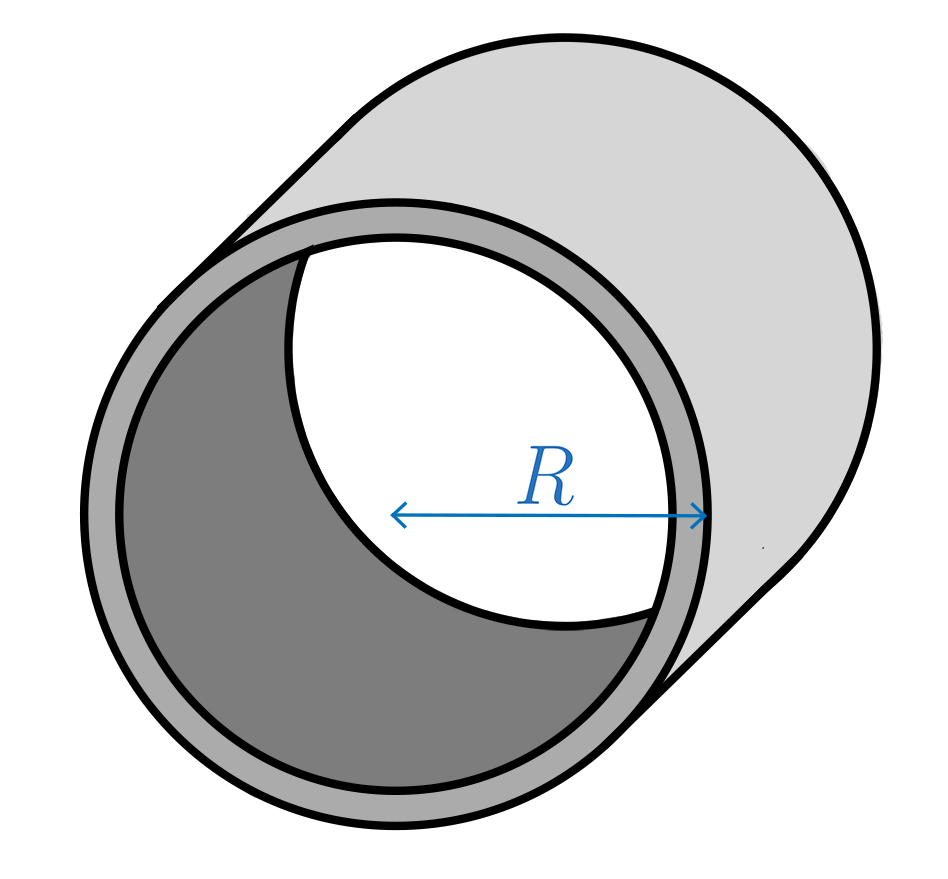
\includegraphics[scale=.5]{fig_sylinderskall-cp1.png}
\captionof{figure}{Illustrasjon av et sylinderskall med radius $R$}
\end{center}
 
Denne klassen skal også beregne og returnere syldinerskallets treghetsmoment. Men i dette tilfellet kan programmet ditt bruke det som allerede har blitt regnet fra klassen i b). Det er nemlig slik at treghetsmomentet til et sylinderskall om sitt massesenter er funnet til å være
\[
I = MR^2
\]
 
Derfor kan denne klassen regne ut sitt treghetsmomentet ved å først regne ut treghetsmomentet til en sylinder, for så gange resultatet med 2. 
 
Lag en instans av denne klassen med $M = 5$ kg og $R = 0.75$ m og skriv ut dets treghetsmoment.
 
\textbf{Bemerkning: } Her er det meningen at du skal skrive ganske så lite kode i denne deloppgaven. Det blir veldig lite kode dersom du utnytter arv til det fulle! 
 
Filnavn: \texttt{Moment\_of\_inertia.py}
\end{document}
 
 

